\chapter{Revisão}\label{revisão}

A importância das técnicas de controle e automação aplicadas a qualquer processo industrial cresceu drasticamente nos últimos 20 anos, sendo atualmente indispensáveis para garantir a qualidade e segurança dos produtos e torná-los competitivos no mercado internacional. Apesar desta importância global, os investimentos são concentrados nos países mais desenvolvidos e em alguns países asiáticos, sendo toda a América do Sul responsável por apenas 4,9 \% dos investimentos tecnológicos em 2010 \citep{future-trends}.

Na indústria de alimentos, os processos envolvem a manipulação de materiais biológicos (alimento), que terão suas propriedades físicas e químicas alteradas na linha de produção. Para controlar estas propriedades, o uso de sistemas de controle automatizados que respondam em tempo real (baseado no conhecimento das propriedades e características físicas do sistema) garante  uma melhora na qualidade do produto, segurança alimentar, menos desperdício de produtos, maior produção e segurança para os trabalhadores.
	
Para que isto possa ocorrer, é necessário implementar um sistema de controle e automação especificamente desenhado para o processo em questão, levando em consideração um modelo matemático do processo e a utilização de sensores e sistemas de medidas em tempo real, dando mais confiabilidade ao sistemas. 

\section{Controle e Automação na Indústria de Alimentos}\label{controle_e_automacao}
 
A implementação de um processo de controle e automação industrial tem como objetivos gerais aumentar a produtividade, reduzir as perdas de produto e aumentar a padronização do produto final. No entanto, na indústria alimentícia, o controle do processamento de alimentos tem algumas particularidades que a diferenciam das demais áreas. Segundo \citet{food-processing-control}, as necessidades específicas que a indústria de alimentos deve considerar são:

\begin{itemize}
  \item Aumento na higiene do processo de produção.
  \item Diminuição dos efeitos da variabilidade natural intrínseca dos produtos alimentícios.
  \item Diminuição dos efeitos perecíveis atribuídos a manipulação industrial.
  \item Padronização das propriedades sensoriais do produto final, garantindo a padronização e qualidade. 
\end{itemize}

\subsection{Controle de processo}

Monitorar parâmetros físicos e químicos através de sensores e utilizar instrumentação eletrônica para que os dados coletados possam ser interpretados e tratados é o passo inicial para que possa ser implementado um sistema de controle. Na indústria de alimentos, os parâmetros mais comuns que necessitam de monitoramento são a temperatura, umidade, ph, pressão, peso, volume, cor, forma e composição. Portanto, são necessários sensores adequados para medir estes parâmetros, de forma que este seja inócuo ao alimento, suporte as adversas condições do processo (temperatura, pressão e etc), possua uma baixa resposta no tempo em comparação com o tempo do processo e seja confiável \citep{process-monitoring-online}.

Uma vez escolhidos os sensores e instrumentação adequados, é delineado o sistema de controle. Ainda segundo \citet{process-monitoring-online}, controle é mais um problema estratégico do que um problema de hardware ou software e ele está na intersecção entre a instrumentação, métodos de produção, automação e aspectos bioquímicos do alimento. Por isto, o sistema de controle deve ser feito levando em consideração o ponto de vista de três áreas de engenharia: A engenharia de Alimentos, a Engenharia de Processo e a Engenharia de Controle.

Os processos industriais, do ponto de vista do produto, podem ser separados em processos de fluxo contínuo e descontínuo. Na indústria de alimentos, devido à especificidade de algumas etapas como esterilização, descanso, fermentação e cozimento, a realidade é mais complexa e na maioria das vezes o que existe é um combinado de processos contínuos e descontínuos \citep{food-processing-control}.  

O controle de processos térmicos em alimentos geralmente consiste em manter condições de operações específicas que já foram pré-determinadas por experimentos de penetração de calor e que garantem que as exigências de saúde alimentar sejam satisfeitas. Caso não haja um sistema de controle, quando ocorre algum desvio no processo e as condições de operação não são garantidas, é necessário corrigir o processo alterando o tempo para compensar, fazendo com que sejam gerados produtos fora da especificação sensorial \citep{advances-intelligent}. Sistemas inteligentes buscam alterar as condições de controle em tempo real para garantir que o alimento passe pelas condições pré-determinadas mesmo com perturbações externas.

Independente do tipo de fluxo, os processos podem ter três estados possíveis: Estacionário, Transiente e Controlado. No estado estacionário, se fixarmos as condições de operação, as variáveis objetivo podem ser previstas e estas serão invariantes no tempo. Este tipo de sistema é fácil de ser controlado porque depois de encontrados os parâmetros ótimos de funcionamento, ele não exige nenhuma lógica de controle computacional. O controle de estado estacionário não leva em conta nenhuma perturbação no sistema, pois as alterações nas condições de operação levam a uma alteração ao longo de um tempo até que um novo estado estacionário seja encontrado. Esta alteração no tempo é o estado transiente.

No estado transiente, ocorre uma resposta do sistema a um estímulo, que pode ser alguma alteração nas condições de controle ou uma condição externa. Diferente do estado estacionário, é impossível predizer a resposta do sistema baseado apenas nas condições de operação inicial e portanto é vital que se tenham medidas em tempo real. O estado transiente, como o nome diz, é o estágio intermediário entre duas condições de operação (estados estacionários ou controlados), fato este que ocorre comumente nos processos com alimentos já que estes geralmente possuem várias etapas de ação diferentes, como por exemplo, o pré-aquecimento, cozimento e torra. Portanto, é importante garantir que a mudança e a trajetória entre os dois estados sejam controladas. Este controle pode ser feito através de uma modelagem dinâmica do sistema ou de uma abordagem experimental baseada em autocorreção utilizando os dados dos sensores em tempo real para esta correção. 

O estado controlado é o ideal a ser alcançado no processo. Nele, o processo possui um comportamento que varia no tempo mas de forma controlada e forçada a ter um perfil pré-escolhido. Para se garantir um estado controlado, ou um transiente estável, é necessário implementar um controle com feedback em ciclo fechado, como é ilustrado pela figura \ref{diagrama_controle}, onde as leituras dos sensores são utilizadas como informação para se calcular a resposta dos atuadores. Estes alterarão o sistema, e esta alteração poderá ser medida pelos sensores novamente e este processo será repetido continuamente. 

\begin{figure}[h]
    \centering
       \begin{tikzpicture}
        \node[elli](Processo){Processo};
        \node[block, below of=Processo](Sensores){Sensores};
        \node[block, below of=Sensores](Controle){Controle};
        \node[block, below of=Controle](Atuadores){Atuadores};
        \path[line](Processo.south) edge (Sensores.north);
        \path[line](Sensores) edge (Controle);
        \path[line](Controle) edge (Atuadores);
        \path[line](Atuadores.east) edge[bend right] (Processo.east);
    \end{tikzpicture}
    \caption{Diagrama mostrando o sistema de controle }
    \label{diagrama_controle}
\end{figure}

\subsection{Controle PID}

O controle Proporcional Integral e Derivativo (PID) é o a estratégia de controle em ciclo fechado mais utilizada na indústria. Segundo \citet{pid}, estima-se que mais de 90\% dos controles em loop fechado utilizem alguma variante do controle PID. Este controle foi desenvolvido antes dos sistemas digitais, com a primeira análise matemática publicada por \citet{pid-Minorsky} e posteriormente implementada com sucesso pela primeira vez para controlar automaticamente a direção de navios da marinha americana na década de 1930 \citep{cite-history-of-control}. 

O uso dos controles PID ou PID modificados é grande devido a sua aplicabilidade geral a sistemas em loop fechado. Ele tem como objetivo levar uma variável do sistema a um valor desejado controlando os atuadores, garantindo que este objetivo seja atingido da forma mais rápida possível com suavidade. Apesar de garantir estabilidade em todos os casos, ele pode não fornecer o controle ótimo em casos extremos do sistema.

No controle PID, é realizada uma tentativa de minimizar o erro, diferença entre o valor medido e o desejado para uma variável do sistema, ajustando o processo por meio de atuadores, assim como ilustrado na figura \ref{diagrama_controle}. O valor deste ajuste, que será inserido no sistema é dependente de três parâmetros, o Parcial, o Integral e o Derivativo, dando o nome ao controle. Na equação \ref{eq:pid} temos o formato geral da resposta do controlador PID.

\begin{equation}\label{eq:pid}
u\left(t\right)=\ K_P * e\left(t\right)+\ K_I\int^t_0{e\left(t\right)dt}+\ K_D\frac{d}{dt}e\left(t\right) 
\end{equation}
Onde $e(t)$ representa o erro, que é a diferença entre o valor desejado e o medido, e $K_P$, $K_I$ e $K_D$ são os parâmetros ajustáveis do controle. Alterações nestes parâmetros modificam o caráter do controle e devem ser encontrados os melhores valores para cada sistema específico.

O termo proporcional dá uma resposta ao sistema que é diretamente proporcional ao erro. Quando um controle contém apenas a parte proporcional (com $K_I=0$ e $K_D=0$), sempre há um erro no regime contínuo, já que  $u(t)$ diminui quando $e(t)$ diminui. Este erro pode ser reduzido aumentando o valor de $K_P$, porém quanto maior for este termo, mais rápido o sistema chegará ao valor desejado, no entanto o sistema poderá oscilar, podendo levar a instabilidade. Na figura \ref{fig:pid_respostal}, podemos ver o efeito de vários valores de $K_P$, mantendo $K_I$ e $K_D$ constantes.

\begin{figure}[H]
\centering
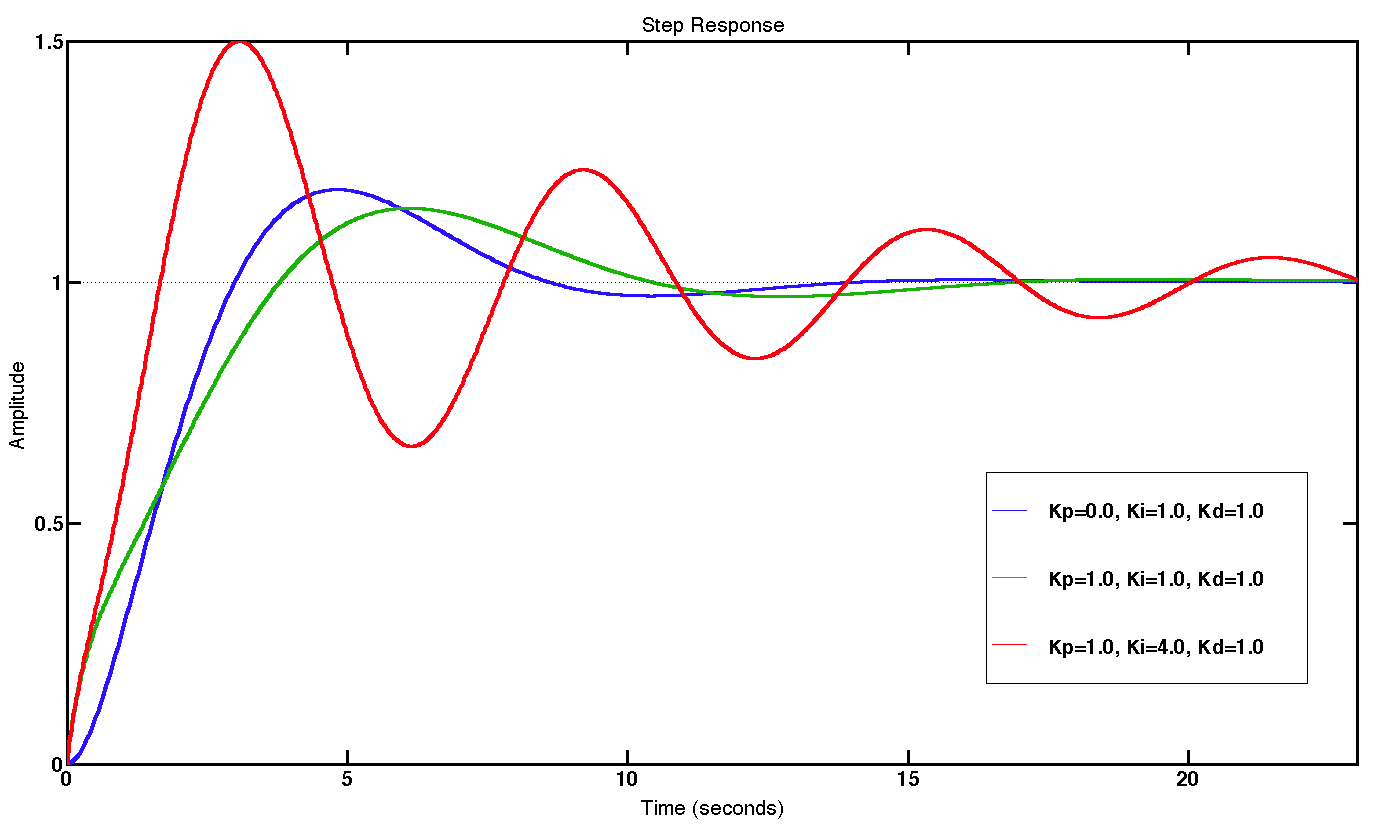
\includegraphics[width=\textwidth]{Figuras/pid_resposta}
\caption{Resposta do sistema em função dos parâmetros $K_p$, $K_i$ e $K_d$}
\label{fig:pid_respostal}
\end{figure}

O termo Integral atua na resposta de forma proporcional tanto ao valor do erro como ao tempo de duração deste erro, já que, como pode ser observado na equação \ref{eq:pid}, $\int^t_0{e\left(t\right)dt} $  é a área do gráfico do valor do erro em função do tempo. Os efeitos do termo $K_I$ no sistema são similares do $K_P$, também podendo levar a oscilações e instabilidades no sistema caso este seja muito alto. Como este termo responde ao erro acumulado, não existe o problema de baixa atuação quando $e(t)$ é pequeno e, portanto não leva a efeitos de erro residual no estado estacionário.

O termo derivativo responde em função da variação do erro $e(t)$ em função do tempo. Por isto, ele prevê a posição futura de $e(t)$ e com isto diminui o tempo que o sistema demora para chegar ao estado estacionário. Este termo deve ser empregado com cuidado pois em situações não ideais, as medidas das variáveis de interesse do sistema estejão sujeita a erros e flutuações como ruídos. Tais erros de medida podem gerar um grande valor da derivada de $e(t)$ e portanto gerar instabilidade no sistema. Por este motivo, sempre é ideal que os sensores possuam uma instrumentação eletrônica adequada, com filtros que evitem este problema.

\subsection{Automação}

Para que os conceitos de controle discutidos previamente possam funcionar em tempo real, as ações devem ser tomadas automaticamente pelo sistema. Portanto a automação é muito mais que uma forma de reduzir o número de trabalhadores braçais. 
Segundo \citet{process-monitoring-online}, os objetivos particulares da indústria de alimentos para a utilização de automação são: 

\begin{itemize}
  \item Qualidade e Confiabilidade.
  \item Segurança Alimentar.
  \item Flexibilidade e Manutenção.
  \item Implementação. 
  \item Aquisição de dados.
\end{itemize}

A qualidade, a confiabilidade e a segurança alimentar já foram discutidas nos benefícios do controle de processo. A flexibilidade e a manutenção são facilitados pela automação, pois numa planta de produção de alimentos, muitos produtos dividem os mesmos equipamentos, portanto a vantagem está em alterar facilmente o sistema para a produção de vários produtos. 

A aquisição de dados ajuda a melhorar o sistema, observando as respostas dos atuadores em várias circunstâncias e verificando os pontos que podem ser aprimorados. O monitoramento dos dados pode servir também como uma forma de alerta para evitar problemas na produção.


\section{Modelagem Matemática e Simulação na Indústria de Alimentos}\label{diffinitas}

A modelagem matemática é a descrição de um sistema real através de equações matemáticas, de forma que, através destas equações possam ser entendidos os efeitos de diferentes componentes do sistema bem como prever o comportamento deste diante de diferentes cenários. A modelagem matemática é a base das ciências naturais, das ciências sociais e da engenharia, já que podem ser testadas, validadas ou refutadas, passando pelo crivo do método científico. Do ponto de vista da Engenharia, o objetivo é analisar e otimizar sistemas, sendo que a descrição matemática do mesmo possibilita que testes sejam feitos através de simulações, economizando tempo e dinheiro. 

Na indústria de alimentos, os principais sistemas específicos a serem modelados são os relacionados a segurança alimentar, como crescimento bacteriano \citep{bacteriano}, os processos de contaminação \citep{contaminacao} e o processo de aquecimento/cozimento de alimentos, já que estes representam um alto gasto energético \citep{modelling-heat-bread} e pequenas alterações no perfil de temperatura do alimento podem  significar grandes mudanças sensoriais e perda do produto \citep{computer-aid}. 

Como o perfil de temperatura é extremamente importante para a qualidade do produto final, muitos estudos foram realizados com o intuito de modelar o processo de aquecimento em fornos. \citet{bread-baking} estudaram o processo interno de assamento levando em consideração o transporte de calor e de massa que ocorrem no interior do forno e dentro do alimento. O aquecimento do forno também foi estudado por \citet{modelling-heat-bread}, que estudaram os processos de transferência de calor e massa que ocorrem dentro de um forno linear tipo esteira com áreas de aquecimento inferior e superior e zonas de exaustão de ar. Tal tipo de forno é o mais comum na produção de pães e biscoitos e por este motivo este tipo de estudo ajudou a projetar fornos mais eficientes e que garantam o perfil de temperatura de forma mais adequada. Ainda em fornos tipo esteira, \citet{numerical-gas-flow} estudaram a velocidade do gás e o processo de convecção e \citet{cfd-modeling} realizaram simulações de dinâmica de fluido para resolver as equações do processo térmico dentro do forno.

\subsection{Transferência de Calor}

O processo de transferência de calor pode ser modelado aplicando um dos princípios mais básicos da Física, a conservação da Energia (E). O problema geral consiste em resolver a equação advinda da conservação de Energia para encontrar a temperatura em todos os pontos do sistema em função do tempo, ou seja, encontrar $T(x,y,z,t)$. Utilizando o princípio da conservação de Energia à um elemento infinitesimal de área podemos encontrar tal relação. Desta forma, podemos escrever a equação \ref{eq:energia}:

\begin{equation}\label{eq:energia}
E_{adicionada} = E_{entra} - E_{sai} + E_{'gerada'}
\end{equation}

Onde a Taxa de acúmulo de Energia é a derivada parcial da Energia em relação ao tempo e pode ser relacionada a temperatura através do Calor Específico pela equação \ref{eq:taxa-acumulo}.

\begin{equation}\label{eq:taxa-acumulo}
\frac{\partial U}{\partial x} \cdot m = \rho \cdot c_{p} \cdot \frac{\partial T}{\partial t}
\end{equation}

Onde $U$ é a energia interna por unidade de massa, $m$ é a massa, $\rho$ a densidade e $c_p$ é o calor específico à pressão constante.

A quantidade de Energia que entra menos a que sai em um elemento infinitesimal, em coordenadas cartesianas pode ser escrita utilizando a expansão em Série de Taylor (equação \ref{eq:taxa-entra-sai}), utilizando apenas o termo de primeira ordem.

\begin{equation}\label{eq:taxa-entra-sai}
E_{adicionada} = - ( \frac{\partial q_x}{\partial x} \cdot dx + \frac{\partial q_y}{\partial y} \cdot dy + \frac{\partial q_z}{\partial z} \cdot dz )
\end{equation}

Levando em consideração que o calor $q_x = -k \cdot (dy \cdot dz) \cdot \frac{\partial T}{\partial x}$, e que $q_y$ e $q_z$ tem o mesmo formato, podemos substituir na equação \ref{eq:energia} e então temos a equação \ref{eq:diferenca-final}.

\begin{equation}\label{eq:diferenca-final}
E_{entra} - E_{sai} = \frac{\partial}{\partial x} \cdot (k \cdot \frac{\partial T}{\partial x}) + \frac{\partial}{\partial y} \cdot (k \cdot \frac{\partial T}{\partial y}) + \frac{\partial}{\partial z} \cdot (k \cdot \frac{\partial T}{\partial z})
\end{equation}

Por último, temos o termo de “geração” de energia (equação \ref{eq:gerada}), que pode ser decorrente de reações químicas, sendo positivo para exotérmicas e negativo para endotérmicas ou também energia eletromagnética absorvida, como por exemplo micro-ondas. 

\begin{equation}\label{eq:gerada}
E_{gerada} = \dot{q}
\end{equation}

Com isto, temos a equação geral da transferência de calor, que em coordenadas cartesianas é dada pela equação \ref{eq:geral}.

\begin{equation}\label{eq:geral}
\rho \cdot c_{p} \cdot \frac{\partial T}{\partial t} = \frac{\partial}{\partial x} \cdot (k \cdot \frac{\partial T}{\partial x}) + \frac{\partial}{\partial y} \cdot (k \cdot \frac{\partial T}{\partial y}) + \frac{\partial}{\partial z} \cdot (k \cdot \frac{\partial T}{\partial z}) +  \dot{q}
\end{equation}

Para se encontrar $T(x,y,z,t)$ deve-se resolver a equação \ref{eq:geral}, aplicadas as condições conhecidas do problema em questão, que são chamadas condições de contorno. Porém, como a equação \ref{eq:geral} é uma EDP (Equação Diferencial Parcial), na maioria dos casos reais ela não pode ser resolvida analiticamente e por isto algum tipo de aproximação deve ser feita. 

Uma forma de se revolver este tipo de problema é nos casos em que alguma simetria, geométrica ou de condições de contorno, possibilitem algum tipo de solução analítica. Outra maneira de contornar o problema da resolução da EDP é desconsiderar termos menos significativos, que podem muitas vezes facilitar muito a solução da equação. Um exemplo clássico é a solução da equação de calor no estado estacionário, onde é considerado que  variação do perfil de temperatura em função do tempo é desprezível e portanto a solução que se quer encontrar, $T(x,y,z,t)$, passa a não ser mais função de t e então temos $T(x,y,z)$. Com isto, a equação \ref{eq:geral} é drasticamente simplificada já que $\frac{\partial T}{\partial t} = 0$ e então temos a equação \ref{eq:simplificada}.

\begin{equation}\label{eq:simplificada}
 k \cdot (\frac{\partial^2}{\partial x^2} + \frac{\partial^2}{\partial y^2} +  \frac{\partial^2}{\partial z^2}) T + \dot{q} = 0 
\end{equation}

Mesmo com a  equação \ref{eq:simplificada}, dependendo de quem for $\dot{q}$ e também da geometria, pode não ser possível resolver o problema analiticamente. Nestes casos, existem vários métodos computacionais que podem ser utilizados.

\subsection{Simulação de Processos Térmicos}

Como na maioria dos casos reais não existe uma solução analítica para a equação da transferência de calor, os métodos numéricos são comumente utilizados para se obter uma aproximação satisfatória das equações. Existem vários métodos computacionais que podem ser utilizados, como por exemplo o método dos elementos finitos, das diferenças finitas e Lattice Boltzman. Além destes métodos numéricos, outra forma de encontrar a solução da equação da transferência de calor é utilizando Eurística, baseando-se em conhecimento experimental prévio do sistema ou em princípios de Mínima Ação. Neste tipo de método podemos destacar  as Redes Neurais e o Algoritmo Genético, respectivamente.

\subsubsection{Diferenças Finitas}

O método das diferenças finitas é uma técnica utilizada para encontrar soluções aproximadas de uma ou de um conjunto de equações diferenciais. Basicamente, o método consiste em substituir a derivada de uma função pela equação \ref{eq:derivada}, utilizando o teorema fundamental do cálculo, com um valor pequeno de $\Delta x$. Desta forma, quanto menor for o valor de $\Delta x$, maior será a precisão do cálculo uma vez que o limite de $\Delta x$ tendendo a zero resulta no valor exato da derivada. 

\begin{equation}\label{eq:derivada}
\frac{\mathrm{d} }{\mathrm{d} x}y(x) = \frac{y(x + \Delta x) - y(x)}{\Delta x}
\end{equation}

Além disso, o método também discretiza o espaço, em uma série de pontos separados por uma distância $\Delta x$. Desta forma, o resultado é um conjunto de equações não diferenciais que podem ser resolvidas para encontrar a solução discretizada da equação.

Quanto menor for $\Delta x$, maior será a precisão do método, no entanto maior será a quantidade de equações e mais demorado será para encontrar a solução.

Depois que $y(x)$ foi discretizado em $k$ valores ($y_1$, $y_2$, ..., $y_k$), o conjunto de equações gerado pelo método tem o formato da equação \ref{eq:dif-discreta} no caso unidimensional e o conceito é similar para duas ou três dimensões. O conjunto de equações acopladas deverá ser resolvido para se encontrar a temperatura em todos os pontos num instante t. 

\begin{equation}\label{eq:dif-discreta}
y_k = \frac{y_{k+1} + y_{k-1} + \dot{q_k} \cdot (\Delta x)^2}{2}
\end{equation}

Como geralmente existe uma grande quantidade de equações, vários métodos de resolução podem ser aplicados, com vantagens e desvantagens que dependem da geometria, quantidade de dimensões e tipo de condições de contorno presentes no problema. As principais a serem destacadas são o método de Jacobi, Gauss-Seidel, Sucessive Over-Relaxacion (SOR) e o método direto. 

No método direto, é montada uma equação matricial no formato $ \mathbf{A} \cdot \mathbf{x} = \mathbf{B}$, onde $\mathbf{A}$ é a matriz dos coeficientes das equações acopladas, $\mathbf{x}$ é a matriz das incógnitas (temperatura) e $\mathbf{B}$ é uma matriz conhecida de valores dada pelas condições de contorno do problema e para o caso unidimensional, o formato da equação matricial é dado pela equação \ref{eq:matricial}, onde foi escolhido k=5 para exemplificar o problema. 

\begin{equation}\label{eq:matricial}
 \begin{bmatrix}
    -2 & 1 & 0 & 0 & 0  
\\  1 & -2 & 1 & 0 & 0
\\  0 & 1 & -2 & 1 & 0
\\  0 & 0 & 1 & -2 & 1
\\  0 & 0 & 0 & 1 & -2
\end{bmatrix}  \cdot \begin{bmatrix}
    T_1 
\\  T_2
\\  T_3
\\  T_4
\\  T_5
\end{bmatrix} = -(\Delta x)^2  \begin{bmatrix}
    \dot{q}_1 
\\  \dot{q}_2
\\  \dot{q}_3
\\  \dot{q}_4
\\  \dot{q}_5
\end{bmatrix} - \begin{bmatrix}
    T_{esquerda}
\\  0
\\  0
\\  0
\\  T_{direita}
\end{bmatrix}
\end{equation}
Onde A e B representam as temperaturas conhecidas nas laterais esquerda e direita de $T_1$ e $T_5$ respectivamente e $\dot{q_1}$, ..., $\dot{q_5}$ representam o calor sendo adicionado ou removido no instante t nos pontos discretizados do eixo x.

O conhecimento da temperatura nas laterais, que é uma codição de contorno chamada condição de Dirichlet, e o conhecimento do calor adicionado no sistema, que é uma condição de contorno de Neumann, precisam ser conhecidas para se encontrar a solução particular do sistema.

Para encontrar a matriz das incógnitas, é preciso simplesmente encontrar a inversa de $\mathbf{A}$. Este processo pode ser computacionalmente custoso para matrizes muito grandes porém como a matriz $\mathbf{A}$ sempre é uma matriz esparsa, este problema pode ser contornado. No caso unidimensional, já que segundo a equação \ref{eq:dif-discreta}, os elementos desconhecidos $T_a$ estão relacionados apenas com os seus vizinhos $T_{k+1}$ e $T_{k-1}$,  a matriz $\mathbf{A}$ é sempre tridiagonal, o que facilita muito a resolução do problema \citep{tridiagonal}, já que reduz o número de iterações da ordem de $n^3$ para $n$, se considerarmos uma matriz $n \times n$. Para o caso 2D e 3D, teremos matrizes com blocos tridiagonais, simetria que também ajuda na inversão da matriz.

Além do método de resolução direta, existem formas iterativas de se resolver o conjunto de equações acopladas. Tanto o método de Jacobi, Gauss-Seidel e SOR consistem em resolver ponto a ponto as equações, partindo de um "chute inicial" para a temperatura. Este cálculo é reiterado até que os valores da temperatura atinjam uma estabilidade e não se alterem mais. 

Os três métodos citados acima variam na forma com que é feita a resolução das equações. No método de Jacobi (equação \ref{eq:jacobi}), o calculo de $T_k^i$ é dado em função de  $T_{k+1}^{i-1}$ e $T_{k-1}^{i-1}$, ou seja, em função da iteração passada. 

\begin{equation}\label{eq:jacobi}
T_k^i = \frac{T_{k+1}^{i-1} + T_{k-1}^{i-1} + \dot{q_k} \cdot (\Delta x)^2}{2}
\end{equation}
Onde $i$ representa a iteração e $T_k^1$, é um "chute" inicial da temperatura para todo $k$. A equação \ref{eq:jacobi} é resolvida para todos os valores de $k$, repetidamente para $i=2$, $i=3$, e assim por diante até que não haja mais alterações significativas nos valores de $T_k$ em relação a iteração anterior, indicando que o algoritmo convergiu e foi encontrada a solução de $T_k$ para todo $k$.

O método de Gauss-Seidel (equação \ref{eq:gauss-seidel}), é um aprimoramento do anterior, e o cálculo de $T_{k}^i$ é feito em função de $T_{k+1}^i$ e $T_{k-1}^i$, e não da iteração anterior ($i-1$), o que acelera o processo de convergência. 

\begin{equation}\label{eq:gauss-seidel}
T_k^i = \frac{T_{k+1}^{i} + T_{k-1}^{i} + \dot{q_k} \cdot (\Delta x)^2}{2}
\end{equation}

No método SOR, a atualização do valor $T_k^i$ leva em conta também um parâmetro chamado parâmetro de relaxação que aumenta a velocidade de convergência. Primeiramente, é calculada a diferença entre $T_k^{i-1}$ e $T_k^i$ encontrado pelo método de Gauss-Seidel. Essa diferença é então amplificada pelo fator $w$, o parâmetro de relaxação, sendo que $ 1 < w < 2$. Finalmente o valor $T_k^i$ real é encontrado, como é mostrado na equação \ref{eq:sor}.

\begin{equation}\label{eq:sor}
T_k^i(sor) = T_k^{i-1} + w \cdot ( T_k^i(Gauss-Seidel) - T_k^{i-1} )
\end{equation}


\section{Sistemas Embarcados}\label{embarcados}

Sistemas embarcados são dispositivos eletrônicos com poder computacional que fazem parte de um sistema mecânico/eletrônico maior. Estes dispositivos interagem com outras partes do sistema realizando operações lógicas em tempo real, assim como um PC (computador pessoal), porém os periféricos de entrada e saída não são de propósito geral e cada sistema embarcado é feito para a sua função específica e, portanto geralmente possui menor custo, tamanho e gasto energético. Eles são encontrados em quase todos os dispositivos eletrônicos atuais, desde controles remotos de televisão, televisões, rádios, semáforos, radares, fornos de micro ondas e etc.

Dentro da indústria de alimentos, os sistemas embarcados mais importantes são os que controlam o processo de produção. Estes sistemas devem estar conectados aos sensores e a outros sistemas da indústria, processando os dados recebidos e tomando as decisões de controle que são enviadas aos atuadores. As alternativas de sistemas embarcados para este tipo de controle são os CLP’s (Controles Lógico Programáveis), microcontroladores, computadores e sistemas mistos com processamento distribuído. Segundo uma pesquisa de \citet{survey-automation}, 88 \% das indústrias de alimentos utilizam os CLP’s como principal forma de controle e em apenas 6 \% predominam sistemas distribuídos. Esta pesquisa também revelou que uma grande gama de marcas e sistemas comerciais são utilizados, inclusive dentro de uma mesma empresa, o que dificulta uma integração mais inteligente dentro do sistema.

Apesar do grande uso de CLP’s dentro das indústrias de alimentos,  estes dispositivos não tiveram a mesma evolução que os computadores portáteis e dispositivos móveis tiveram nos últimos 15 anos, com um grande aumento no processamento e redução no preço. Por este motivo o desenvolvimento de sistemas de controle baseados em microcontroladores tem crescido muito, com placas que podem realizar as mesmas operações com tamanho e custo reduzido \citep{clp-microcontrolador}. Para controles mais complexos, que exijam um maior processamento de dados, os sistemas de computação de baixo custo baseados em hardwares similares a tablets e celulares também é uma alternativa emergente. 

\subsection{Microcontroladores}

Microcontroladores são pequenas unidades de processamento que possuem todos os seus elementos de processamento e memória em um único chip e, portanto podem operar sem a necessidade de periféricos. Esta é a principal diferença entre um microcontrolador e um microprocessador, como os que são encontrados nos computadores. Por possuir todas as unidades em um único chip, seu processamento e memória são em geral muito inferiores a de um computador, porém as vantagens estão na quantidade de energia utilizada, tamanho e robustez. 

Os microcontroladores surgiram na década de 1970 e tiveram um enorme avanço até o momento. Atualmente, existem centenas de empresas que produzem microcontroladores e suas especificações variam de acordo com o objetivo do mesmo dentro do sistema, podendo ir de chips minúsculos e baratos com velocidade da ordem de kHz e apenas um pino digital de entrada e saída a microcontroladores ARM (Advanced RISC Machine – Máquina RISC Avançada), que possuem processamento e arquitetura superior aos microcontroladores RISC tradicionais, atingindo processamento da ordem de GHz. 

\subsubsection{Arduino}

Dentro deste conceito de hardware livre surge a plataforma Arduino (figura \ref{fig:arduino}). Esta plataforma foi concebida em 2005 por uma equipe sediada na Itália liderada pelo pesquisador Massimo Banzi, que queria ensinar eletrônica e programação de computadores a alunos de design, para que eles usassem em seus projetos de arte, interatividade e robótica \citep{arduino-araujo}. O intuito da equipe era desenvolver uma plataforma para introduzir os conceitos de eletrônica e programação para leigos de forma intuitiva, simplificada e de baixo custo \citep{arduino-barrett}.

\begin{figure}[H]
\centering
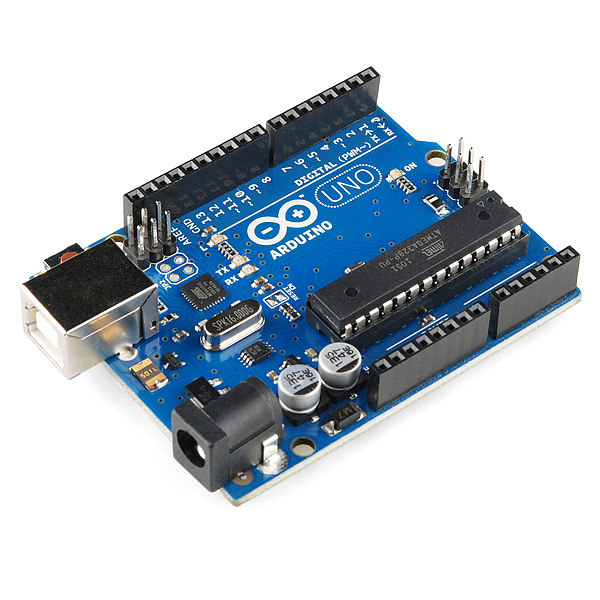
\includegraphics[width=\textwidth]{Figuras/arduino}
\caption{Arduino Uno R3 – Principal placa da plataforma Arduino, com Atmega328pu e Comunicação USB}
\label{fig:arduino}
\end{figure}

O Arduino é uma plataforma de placas microcontroladoras que permite entrada de dados de sensores e comunicação digital e saídas de dados e sinal elétrico que possibilita acionar motores, LEDs e outros dispositivos. A principal placa da linha Arduino, o Arduino Uno utiliza um microcontrolador \textregistered{Atmel} da linha Atmega com um oscilador de 16 MHz externo, um regulador de tensão de 5 V, botão de reset, plugue de alimentação, pinos conectores, e alguns LEDs para facilitar a verificação do funcionamento. A conectividade é feita diretamente por uma porta USB, tanto para gravar os programas quanto para comunicação serial. Além disso, a porta USB pode também fornecer a alimentação de 5 V para a placa.

A gravação dos programas na placa é controlada por um chip que faz a conversão USB para Serial, sendo nos primeiros modelos o CHIP FT232RL, que na terceira revisão do Arduino UNO foi substituído por um microcontrolador Atmega16U2, que tem o papel exclusivo de ser a interface entre a porta USB e o Arduino \citep{arduino-testes}. Este conceito é uma das chaves do sucesso da plataforma, já que a gravação dos programas pode ser feita diretamente na placa, não exigindo um gravador externo como a maioria dos microcontroladores do mercado. Isto viabilizou a utilização de microcontroladores por pessoas que não tem acesso a um laboratório de eletrônica.

A programação do microcontrolador utiliza uma interface integrada de desenvolvimento (IDE) baseada na IDE da linguagem Processing, que é uma versão simplificada (mas não menos poderosa) da linguagem C/C++ \citep{arduino-buechley}. Esta Linguagem foi desenvolvida em 2001 no laboratório de mídia do MIT (Massachusetts Institute of Technology), e esta licenciada sobre a licença GPL e LGPL (General Public License - Licença Pública Geral), sendo completamente open source e cross plataforma, podendo ser utilizado nos sistemas Windows, Linux e Mac OS. O \textit{Processing} foi desenvolvido inicialmente para facilitar o uso de programação por artistas e ensinar programação de forma simples e visual \citep{processing} e pela sua facilidade é utilizado atualmente por milhões de pessoas desde o ensino a prototipagem e produção de softwares.

Outra facilidade da plataforma Arduino é a padronização dos pinos de Entrada e Saída, possibilitando que uma série de circuitos de expansão, chamados de Shields, possam ser utilizados com as placas, dando funções extras ao microcontrolador, como comunicação Bluetooth, wi-fi, GSM, Relês entre outros. Estes Shields, assim como as próprias placas, podem ser produzidos por qualquer companhia já que o Arduino é um hardware livre. Com isto, com a popularização das placas, mais sensores, Shields e periféricos são produzidos para abastecer o ecossistema, o que torna o Arduino ainda mais popular, fazendo disto um ciclo positivo \citep{arduino-livro}. O mesmo ciclo ocorre com a disponibilização de projetos com código aberto e dessa forma, quanto maior for o número de usuários da plataforma, maior será a quantidade de projetos livres e suporte disponíveis para o ecossistema.

\subsection{Computação de Baixo Custo}

Com o avanço e desenvolvimento de novos hardwares com mais memória e processamento e, principalmente devido à corrida tecnológica dos dispositivos móveis, surgiu nos últimos anos a computação de ultra baixo custo (Ultra Low Cost Computing – ULCC), que basicamente utiliza o hardware de smartphones e periféricos de entrada e saída em uma única placa \citep{low-cost-computing}. Vários projetos tem se desenvolvido neste sentido, entre eles podemos citar o Beaglebone, Galileu Board, Raspberry Pi, Arduino Yun e PcDuino. Tais projetos entregam placas de baixo custo (de 20 a 70 dólares) que possibilitam aplicações em várias áreas como automação, robótica, equipamentos médicos \citep{raspberry-pesquisa}, ensino de computação e programação, aquisição dinâmica de dados, servidores web, monitoramento remoto e até controle de satélites \citep{raspberry-embedded}, entre outras aplicações. 

Existem vários modelos de computadores em uma única placa, que diferem nas suas especificações de preço, processamento, sistema operacional e tipo de licença. Levando em conta o preço, licença e a quantidade de usuários, o Raspberry pi é a placa que mais se destaca no mercado atualmente.

\subsubsection{Raspberry Pi}

O Raspberry pi é um computador em uma única placa do tamanho de um cartão de crédito (figura \ref{fig:raspberry}), desenvolvido pela Raspberry Pi Foundation, que se iniciou com o intuito de promover o ensino básico de computação em escolas com baixo custo. O Raspberry Pi, modelo B é produzido em um único chip broadcom BCM2835, com um processador ARM de 700 MHz e 512 Mb de memória RAM. A memória física fica em um cartão SD de até 32 Gb e suporta uma série de sistemas operacionais baseados em Linux e a distribuição oficial da Raspberry Pi Foundation é um Linux Debian chamado wheezy. Este modelo possui duas entradas USB, uma porta Ethernet, uma saida HDMI, uma saída RCA, uma saída de vídeo e oito pinos GPIO (General Purpose Input/Output - Pinos de entrada/saída de propósito geral).

\begin{figure}[H]
\centering
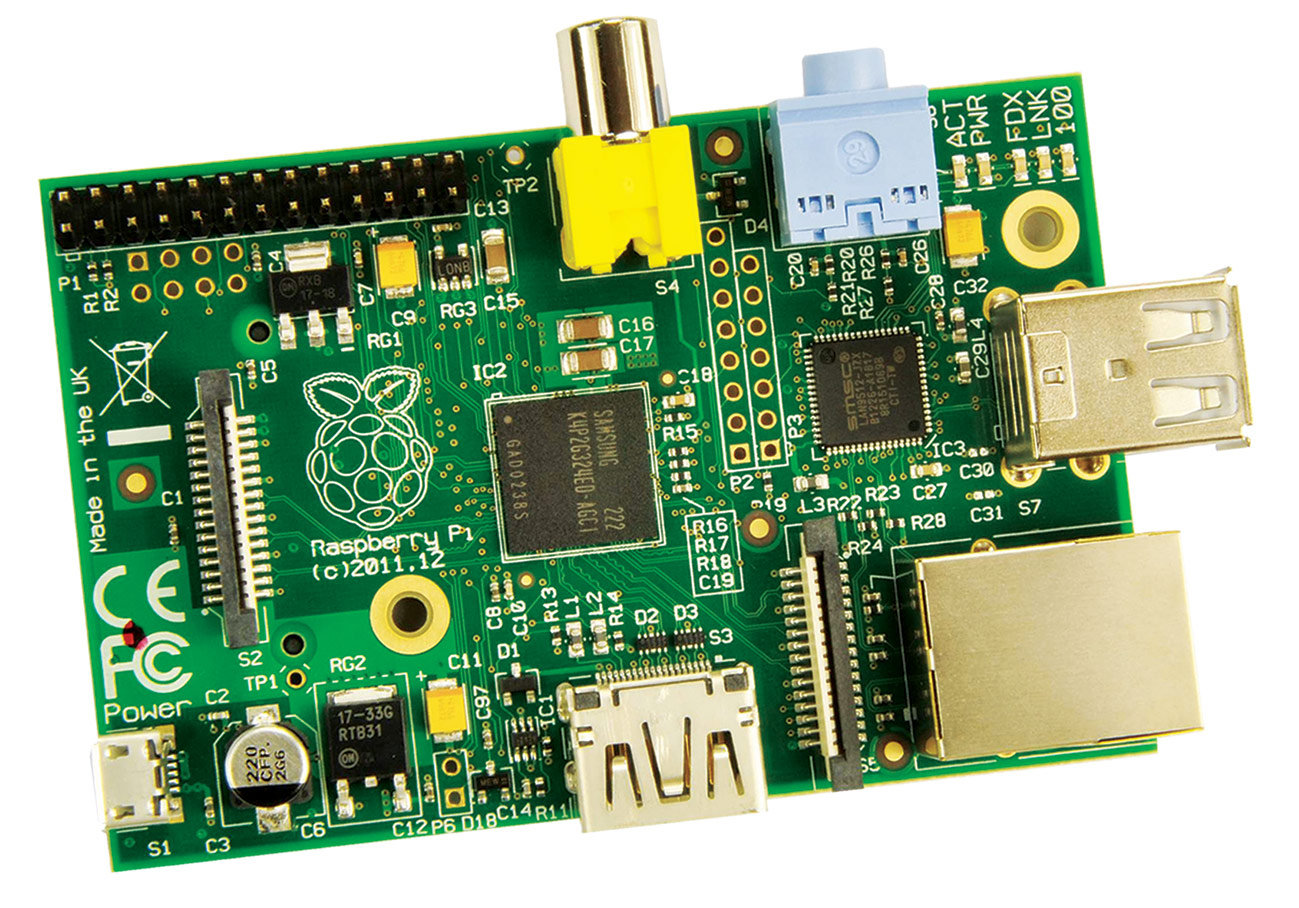
\includegraphics[width=\textwidth]{Figuras/raspberry}
\caption{Raspberry pi – Modelo B}
\label{fig:raspberry}
\end{figure}

O projeto foi concebido em 2006 como uma forma barata e simples de ensinar computação, programação e eletrônica às crianças. Em 2008 o projeto saiu do papel com o modelo A, que possuía 256 Mb de memória RAM (Random Access Memory) e uma entrada USB. Este modelo recebeu um upgrade em 2011, contando agora com uma memória de 512 Mb e duas entradas USB. Por ser um projeto totalmente open-source ele usa uma distribuição Unix com licença GNU além de um hardware aberto. Com isto, o Raspberry Pi ganhou muitos adeptos rapidamente, sendo utilizado atualmente em várias áreas como ensino, processamento e clusters, webservers e uma série de projetos embarcados.

Na área da educação, a placa tem sido utilizada devido ao seu baixo custo (aproximadamente 35 dólares) e também por ser uma maneira mais acessível do usuário entender e manipular o hardware. Nesta ultima década, dispositivos computacionais tem se tornado equipamentos fechados em que o usuário o encara como unidades lacradas de alumínio ou plástico, sem ideia do que esta dentro. Neste sentido, o Raspberry Pi possibilita ao usuário o entendimento a alterações no hardware assim como do software, já que utiliza um Linux que possui várias vantagens didáticas. Baseado nestas ideias, alguns projetos para ensino de computação em comunidades carentes utilizam esta plataforma como uma alternativa barata e poderosa, como por exemplo, o projeto de \citet{raspberry-data}.

Além de projetos educacionais, o Raspberry Pi é utilizado também em projetos de pesquisa de ponta, como por exemplo o satélite CCRMA \citep{raspberry-embedded} que envia placas para controlar pesquisas científicas em satélites. Na área da medicina, existem vários projetos de controle e desenvolvimento de equipamentos baratos \citet{raspberry-pesquisa}.

No novo conceito de IoT (Internet of Things - Internet das Coisas), desenvolvido por Kevin Ashton em 2009, num mundo onde objetos físicos estão integrados a uma rede de informações, os objetos se tornam “inteligentes” e podem interagir com o resto da rede. Neste cenário, computadores pequenos e de baixo custo como o Raspberry Pi são extremamente importantes já que podem servir como unidades móveis de processamento de dados \citep{raspberry-pesquisa} bem como receber e processar dados de sensores numa rede multi-agente \citep{raspberry-data}.









































